\documentclass[../main.tex]{subfiles}

\begin{document}
The alignment algorithm has been thoroughly tested using both synthetic and experimental datasets. Synthetic data is valuable because the ground truth values of the alignment parameters are known. As a consequence, any discrepancy in the output can be attributed as an error of the alignment algorithm. In spite of this, the synthetic data is usually generated using a naive model of the microscope. Therefore, results obtained with synthetic data may not reflect the real performance of the algorithm. To address this issue, the algorithm has also been tested with experimental data.

The datasets used for our tests were selected to reflect proteins with a diverse set of characteristics, such as symmetry, size, pixel size, presence of membrane, flexible parts\dots In total, 4 proteins were elected. Each of these proteins will be tested with both simulated and experimental data.

\subsection{Experimental Data}
The experimental images used in these tests were obtained from \gls{empiar}. \Gls{empiar} is a public archive maintained by the \gls{embl}-\gls{ebi} which provides open access to raw \gls{cryoem} images\cite{iudin2022}. Among other things, this initiative enables testing \gls{cryoem} image processing algorithms with a wide variety of real data.

Some of the selected datasets provided extracted particles, which are the starting point of the alignment algorithm. However, some others only provided micrographs or movies. In those cases, data needed to be processed before being suitable for our use case. This processing was done inside the Scipion framework. Depending on the dataset, movie alignment, \gls{ctf} estimation, particle picking and particle extraction steps needed to be carried out to obtain the desired particles.

To address the fact that the alignment information of the experimental images is not known, these particles were aligned twice using Relion\cite{scheres2021} or Cryosparc\cite{cryosparc}. Then, their outputs were consensuated so that only particles that coincided below a threshold are considered. This gives some amount of confidence to the estimated alignment of the particles, as two independent algorithms coincided in the result. Nevertheless, these parameters do not need to be the ground truth.

\subsection{Synthetic Data}
\Gls{empiar} datasets have one or more atomic models associated to them in the \gls{pdb} archive. The synthetic datasets used to test the algorithm were generated from those atomic models using the Scipion framework\cite{delarosa2016}. This process will mimic the behaviour of the \glspl{tem}.

Atomic models describe the the protein structure with atom coordinates. Therefore, the first step is to render a volume from this model. This can be easily achieved using the \texttt{xmipp3 - convert a PDB} protocol. Then, this volume is projected from all directions using \texttt{xmipp3 - create gallery} protocol, leading to a set of clean projections of the volume. However, these projections do not reflect experimental images due to the absence of noise. Therefore, some amount of \gls{agwn} is added to the images through the \texttt{xmipp3 - add noise particles} protocol to simulate ice particles in the sample. This noise has zero mean and its standard deviation will be selected in such a way that the \gls{snr} of the image is $-10 \si{\decibel}$. Lastly, a \gls{ctf} is applied to the images using \texttt{xmipp3 - simulate CTF} protocol. 

In total, $41219$ projections will be generated from equally spaced orientations. This ensures that the algorithm will be tested with all possible orientations of the protein. Additionally, the particles will be shifted in-plane by a normal distribution of $\sigma=6\si{px}$. Therefore, $95\si{\percent}$ of the images will contain a shift of less than $12 \si{px}$, which is a reasonably high value. Similarly, the defocus parameter of the \gls{ctf} will be uniformly chosen for each particle in the range of $5000 \si{\angstrom}$ to $25000 \si{\angstrom}$.


\subsection{Test proteins}
\subsubsection{EMPIAR-10028}
This acquisition is related to the Plasmodium falciparum protein, which is present in the human malaria parasite\cite{wong2014}\cite{empiar10028}. The dataset is widely used when testing \gls{cryoem} algorithms. In fact, as of May 2023, it has been cited by $28$ publications related to new \gls{cryoem} methods. A visual sample of the particles is displayed in Figure \ref{fig:5:empiar10028}.

\begin{figure}[htbp]
    \centering
    \begin{subfigure}[b]{0.45\textwidth}
         \centering
         \includegraphics[width=\linewidth]{results/datasets/empiar10028/experimental}
         \caption{Experimental images}
    \end{subfigure}
    \hfill
    \begin{subfigure}[b]{0.45\textwidth}
         \centering
         \includegraphics[width=\linewidth]{results/datasets/empiar10028/phantom}
         \caption{Simulated images}
    \end{subfigure}
    \caption{Visual aspect of EMPIAR-10028 data}
    \label{fig:5:empiar10028}
\end{figure}

Parts of this protein are very flexible. This makes particles difficult to align, as the particles can not be fitted properly to the entire volume at once. Moreover the protein is quite large, requiring particle images to be also large ($300 \si{px}$ wide).

As stated earlier, alignment algorithms use particles and a volume as the starting point. Although individual particles are provided in the dataset, these particles were obtained several years ago. Therefore, we preferred to obtain the particles from scratch using modern methods so that we can take advantage of state-of-the-art algorithms.

After performing the angular assignment consensus between two independent Relion refinements, $60210$ experimental particles were left with a discrepancy lower than $1 \si{\degree}$ in the angular assignment and $0.5 \si{px}$ in the shift assignment. These refinements reached a resolution of $4.06 \si{\angstrom}$ in their final volumes. The reconstructed volume can be observed in Figure \ref{fig:5:empiar10028_rec}. We also followed this procedure with Cryosparc (Homogeneous and Non-Uniform refinements) but we were unable to obtain good results.

\begin{figure}[htbp]
    \centering
    \begin{subfigure}[b]{0.3\textwidth}
         \centering
         \includegraphics[width=\linewidth]{results/datasets/empiar10028/XY}
         \caption{XY}
    \end{subfigure}
    \hfill
    \begin{subfigure}[b]{0.3\textwidth}
         \centering
         \includegraphics[width=\linewidth]{results/datasets/empiar10028/XZ}
         \caption{XZ}
    \end{subfigure}
    \hfill
    \begin{subfigure}[b]{0.3\textwidth}
         \centering
         \includegraphics[width=\linewidth]{results/datasets/empiar10028/YZ}
         \caption{YZ}
    \end{subfigure}

    \caption{Central slices of the reconstructed EMPIAR-10028 experimental dataset}
    \label{fig:5:empiar10028_rec}
\end{figure}

\subsubsection{EMPIAR-10061}
The \gls{empiar}-10061 dataset is an acquisition of the $\beta$-galactosidase protein\cite{bartesaghi2015}\cite{empiar10061}. Similarly to the prior dataset, this dataset is also widely used when assessing \gls{cryoem} algorithms, having been cited in $23$ publications related to \gls{cryoem} algorithms. 

The particularity of this dataset is that it has $D2$ symmetry. This is important when aligning, because it reduces the number of possible projection angles. Moreover, each experimental image can be used to fill multiple planes in Fourier space when reconstructing, which usually increases \gls{snr} and resolution.

Contrary to the previous example, Relion's refinement introduced some artefacts. Therefore, Cryosparc's result was used for reference. The refinement reached a resolution of $2.6 \si{\angstrom}$, which is close to the theoretical resolution limit imposed by Nyquist. After consensuating two independent Cryosparc runs, $39682$ particles were kept with a discrepancy lower than $0.2 \si{px}$ in shift assignment and $0.5 \si{\degree}$ in angular assignment. The resulting reconstructed volume can be observed in Figure \ref{fig:5:empiar10061_rec}.

\begin{figure}[htbp]
    \centering
    \begin{subfigure}[b]{0.45\textwidth}
         \centering
         \includegraphics[width=\linewidth]{results/datasets/empiar10061/experimental}
         \caption{Experimental images}
    \end{subfigure}
    \hfill
    \begin{subfigure}[b]{0.45\textwidth}
         \centering
         \includegraphics[width=\linewidth]{results/datasets/empiar10061/phantom}
         \caption{Simulated images}
    \end{subfigure}
    \caption{Visual aspect of EMPIAR-10061 data}
    \label{fig:5:empiar10061}
\end{figure}

\begin{figure}[htbp]
    \centering
    \begin{subfigure}[b]{0.3\textwidth}
         \centering
         \includegraphics[width=\linewidth]{results/datasets/empiar10061/XY}
         \caption{XY}
    \end{subfigure}
    \hfill
    \begin{subfigure}[b]{0.3\textwidth}
         \centering
         \includegraphics[width=\linewidth]{results/datasets/empiar10061/XZ}
         \caption{XZ}
    \end{subfigure}
    \hfill
    \begin{subfigure}[b]{0.3\textwidth}
         \centering
         \includegraphics[width=\linewidth]{results/datasets/empiar10061/YZ}
         \caption{YZ}
    \end{subfigure}

    \caption{Central slices of the reconstructed EMPIAR-10061 experimental dataset}
    \label{fig:5:empiar10061_rec}
\end{figure}

\subsubsection{EMPIAR-10256}
This dataset is  a TRPV5 with calmodulin bound \gls{cryoem} acquisition\cite{dang2019}\cite{empiar10256}. This protein is present in the walls of the cells to exchange calcium with the outside. Due to is nature, the protein is embedded on a membrane, which makes it difficult to align. This is because the membrane is highly flexible and does not have a fixed pattern across particles. To make matters worse, the TPRV5 protein has C4 symmetry, but the calmodulin is not bound symmetrically. Therefore, the ensemble is pseudo-symmetric, producing a set of highly similar but disctinct views.

\begin{figure}[htbp]
    \centering
    \begin{subfigure}[b]{0.45\textwidth}
         \centering
         \includegraphics[width=\linewidth]{results/datasets/empiar10256/experimental}
         \caption{Experimental images}
    \end{subfigure}
    \hfill
    \begin{subfigure}[b]{0.45\textwidth}
         \centering
         \includegraphics[width=\linewidth]{results/datasets/empiar10256/phantom}
         \caption{Simulated images}
    \end{subfigure}
    \caption{Visual aspect of EMPIAR-10256 data}
    \label{fig:5:empiar10256}
\end{figure}

The dataset is provided either in the form of aligned particles or micrographs. For our purposes, the particles were elected as the starting point. These particles were refined using two runs of Cryosparc's Non-Uniform refinement. The angles produced by these refinements were consensuated to obtain $53964$ particles with a discrepancy lower than $1 \si{\degree}$ in angular assignment and $0.5 \si{px}$ in shift assignment. The refinements reached a resolution $3.21 \si{\angstrom}$ on its last iteration and slices of the reconstructed volume can be observed in Figure \ref{fig:5:empiar10256_rec}. The same procedure was used with Relion but the results were worse.

\begin{figure}[htbp]
    \centering
    \begin{subfigure}[b]{0.3\textwidth}
         \centering
         \includegraphics[width=\linewidth]{results/datasets/empiar10256/XY}
         \caption{XY}
    \end{subfigure}
    \hfill
    \begin{subfigure}[b]{0.3\textwidth}
         \centering
         \includegraphics[width=\linewidth]{results/datasets/empiar10256/XZ}
         \caption{XZ}
    \end{subfigure}
    \hfill
    \begin{subfigure}[b]{0.3\textwidth}
         \centering
         \includegraphics[width=\linewidth]{results/datasets/empiar10256/YZ}
         \caption{YZ}
    \end{subfigure}

    \caption{Central slices of the reconstructed EMPIAR-10256 experimental dataset}
    \label{fig:5:empiar10256_rec}
\end{figure}

\subsubsection{EMPIAR-10391}
This dataset refers to a Arabinofuranosyltransferase AftD from Mycobacteria \gls{cryoem} acquisition. This protein is responsible of causing the tuberculosis decease, which kills over 1 million people every year\cite{tan2020}\cite{empiar10391}.

Similarly to the previous example, the dataset is distributed either in the form of movies or a particle stack. As mentioned earlier, the later one suits better our needs, as the input for the alignment algorithm is a particle stack. Figure \ref{fig:5:empiar10391} shows the visual aspect of the dataset. 

\begin{figure}[htbp]
    \centering
    \begin{subfigure}[b]{0.45\textwidth}
         \centering
         \includegraphics[width=\linewidth]{results/datasets/empiar10391/experimental}
         \caption{Experimental images}
    \end{subfigure}
    \hfill
    \begin{subfigure}[b]{0.45\textwidth}
         \centering
         \includegraphics[width=\linewidth]{results/datasets/empiar10391/phantom}
         \caption{Simulated images}
    \end{subfigure}
    \caption{Visual aspect of EMPIAR-10391 data}
    \label{fig:5:empiar10391}
\end{figure}

The aim of the experiment was to test a drug binding to the protein. Hence, the dataset is heterogeneous, this is, some particles may originate from the clean protein and some others may originate from the protein with the drug bound. As the dataset reflects two structures, two atomic models were fitted into it. Consequently, these particles can be used to test if the algorithm is able to distinguish discrete 3D classes. 

Another peculiarity of this experiment is that the protein is embedded in a membrane. The membrane structure is highly flexible and does not follow a specific pattern across particles, making it difficult to align.

Similarly to the prior datasets, two independent Cryosparc refinements were run. Their angular assignments were consensuated to obtain a estimation of the ground truth values. At the end $96256$ particles were kept. These Cryosparc refinements produced a volume with a resolution of $2.9\si{\angstrom}$. Slices of this volume can be viewed in Figure \ref{fig:5:empiar10391_rec}. The same procedure was used with Relion but the results were worse.


\begin{figure}[htbp]
    \centering
    \begin{subfigure}[b]{0.3\textwidth}
         \centering
         \includegraphics[width=\linewidth]{results/datasets/empiar10391/XY}
         \caption{XY}
    \end{subfigure}
    \hfill
    \begin{subfigure}[b]{0.3\textwidth}
         \centering
         \includegraphics[width=\linewidth]{results/datasets/empiar10391/XZ}
         \caption{XZ}
    \end{subfigure}
    \hfill
    \begin{subfigure}[b]{0.3\textwidth}
         \centering
         \includegraphics[width=\linewidth]{results/datasets/empiar10391/YZ}
         \caption{YZ}
    \end{subfigure}

    \caption{Central slices of the reconstructed EMPIAR-10391 experimental dataset}
    \label{fig:5:empiar10391_rec}
\end{figure}

\end{document}